\documentclass[slovene,11pt,a4paper]{article}
%\usepackage{fullpage}
\usepackage[margin=2cm]{geometry}

\usepackage[T1]{fontenc}

\newcommand\sul{{\rm S}}
\newcommand\oxi{{\rm O}}
\newcommand\jod{{\rm I}}


%dodatni paketki:
\usepackage{graphicx}
\usepackage{amsmath,amsfonts,amsthm} %matematicni paket
\usepackage{color} % omogoča barvno pisanje
\usepackage[utf8]
{inputenc}
\usepackage[slovene]{babel} % slovenski jezik/hyphenation
\usepackage{hyperref} %naredi vse povezave rečerenc, kazala,...
\numberwithin{equation}{section} % Number equations within sections (i.e. 1.1, 1.2, 2.1, 2.2 instead of 1, 2, 3, 4)
\numberwithin{figure}{section} % Number figures within sections (i.e. 1.1, 1.2, 2.1, 2.2 instead of 1, 2, 3, 4)
\numberwithin{table}{section} % Number tables within sections (i.e. 1.1, 1.2, 2.1, 2.2 instead of 1, 2, 3, 4)
\usepackage{eurosym} %za znak €
\usepackage{rotating} %za rotiranje slike

\usepackage{mathrsfs}
\usepackage{mathabx} % za kemisjke smeri in naslednje 3 vstrice
\catcode`_=12
\begingroup\lccode`~=`_\lowercase{\endgroup\let~\sb}
\mathcode`_="8000


\usepackage[margin=2cm]{geometry}
\include{template}



\begin{document}
\begin{titlepage}

\newcommand{\HRule}{\rule{\linewidth}{0.5mm}} % Defines a new command for the horizontal lines, change thickness here

\center % Center everything on the page

%----------------------------------------------------------------------------------------
%	LOGO
%----------------------------------------------------------------------------------------

%\includegraphics{Logo}\\[1cm] % Include a department/university logo - this will require the graphicx package
 
%----------------------------------------------------------------------------------------


\includegraphics[width=2cm]{slike/aaa}\\[0.5cm]
 
%----------------------------------------------------------------------------------------
%	NASLOV DELA
%----------------------------------------------------------------------------------------
\textit{Univerza v Ljubljani}\\
\textit{Fakulteta za {\color{red}matematiko in fiziko}}\\[0.5cm]

\emph{Oddelek za fiziko}\\[0.5cm] % Oddelek za fiziko


%----------------------------------------------------------------------------------------
%	TITLE SECTION
%--------------------------------------------------------------------------------------
\HRule \\[0.4cm]
\huge {\bfseries 6. naloga: Luščenje modelskih parametrov: linearni model}\\[0.4cm] % NASLOV SEMINARJA
\HRule \\[0.5cm] 

 \textsc{\large Poročilo pri predmetu modelska analiza 1}\\
 \textsc{\large 2015/2016}\\[1cm] % SEMINASKO DELO
 
%----------------------------------------------------------------------------------------
%	AUTHOR SECTION
%----------------------------------------------------------------------------------------



% If you don't want a supervisor, uncomment the two lines below and remove the section above
\Large \emph{Avtor:}\\
Klemen \textsc{Rahne}\\
28152028\\[2cm]
%----------------------------------------------------------------------------------------
%	DATUM
%----------------------------------------------------------------------------------------

{\large \today } \\[0.5cm] % Date, change the \today to a set date if you want to be precise

	

\end{titlepage}


%----------------------------------------------------------------------------------------
%	KAZALO
%----------------------------------------------------------------------------------------

%\tableofcontents

%----------------------------------------------------------------------------------------
%	ZAČETEK TEKSTA
%----------------------------------------------------------------------------------------

\section{Odziv tkiva}

V farmakologiji merimo odziv tkiva na reagent. V stacionarnem stanju odziv ($y$ - vezava reagenta v odvisnosti od koncentracije reagenta - $x$) opišemo:
\begin{equation}
y=\frac{y_0 x}{x+a} ,
\end{equation}
kjer je $y_0$ nasičeni odziv tkiva in $a$ koncentracija potrebna za odziv, ki je enaka polovici nasičenega. Ker zgornja enačba ni linearna jo preoblikujemo v linearno s transformacijo spremenljivk:
\begin{equation*}
u=\frac{1}{y} \qquad  ;\qquad  v=\frac{1}{x}
\end{equation*}


Parametra $k$ in $n$ določimo tako, da mora biti odstopanje modelske funkcije od podatkov minimalno. V matematičnem zapisu:
\begin{equation}
\label{hi-minimum}
\chi^2 =\sum_{i=1}^N \bigg( \frac{u_{i}- k v_i -n }{\sigma_i} \bigg) ^2 = MIN
\end{equation}
kjer smo vsako merilno točko utežili s velikostjo njene napake $\sigma_i$ (točka, ki ima večjo napako, naj bo manj pomembna). Minimum zgornje enačbe se lahko reši na dva načina: analitično in numerično. Pri numerični metodi je postopek podoben kot pri nelinearni minimizacije, kjer smo iskali parametre, ki nam dajo minimum poljubne funkcije. Analitično reševanje je mogoče le za ti. linearno regresijo, kjer lahko zgornji problem zapišemo v matrično obliko.
\begin{equation}
\vec{a} = A \vec{b}
\end{equation}

V matriki $A$ so shranjene vrednosti spremenljivke $v_i$ in v vektorju $\vec{b}$ sta elementa ravno koeficienta $k$ in $n$ v obliki:
\begin{equation*}
A=
\begin{bmatrix}
    1 & v_1 \\
    1 & v_2 \\
    \vdots & \vdots  \\
    1 & v_N
\end{bmatrix}
\qquad  ;\qquad 
b=
\begin{bmatrix}
    n\\
    k
\end{bmatrix}
\end{equation*}
medtem, ko je v  vektorju $\vec{a} $ zapisana spremenljivka $u_i$:
\begin{equation*}
a=
\begin{bmatrix}
    u_1\\
    u_2\\
    \vdots \\
    u_N
\end{bmatrix}
\end{equation*}
Nadaljujemo, tako da vstavimo v minimizacijsko funkcijo matrično enačbo in jo odvajamo po vektorju $\vec{b}$ in odvod enačimo z $0$. Tako dobimo rešitev za vektor $\vec{v}$:
\begin{equation}
\label{resitev-koeficientov}
\vec{b}=(A^T W A)^{-1} A^T W \vec{a}
\end{equation}
kjer je matrika $W$ utežna matrika, dimenzije $NxN$, ki ima je naslednje oblike:

\begin{equation*}
W=
\begin{bmatrix}
    \frac{1}{\sigma_1^2} & 0 & \dots & 0 \\
    0 & \frac{1}{\sigma_2^2} & \dots & 0 \\
    \vdots & \vdots &  & \vdots  \\
    0 & 0 & \dots & \frac{1}{\sigma_N^2}
\end{bmatrix}
\end{equation*}
Napake posameznega parametra in njihove korelacije dobimo iz matrike:
\begin{equation}
M=(A^T W A)^{-1}
\end{equation}


Za podatke iz datoteke \textbf{farmakoloski.dat} dobomo naslednje vrednosti za koeficientov:
\begin{table}[h]
\centering
\label{tabela-1}
\begin{tabular}{l|l|l|}
\cline{2-3}
                             & \multicolumn{2}{l|}{linearno prilagajanje} \\ \cline{2-3} 
                             & vrednost             & napaka              \\ \hline
\multicolumn{1}{|l|}{$y_0$}  & 104.7               & $\pm$2.5          \\ \hline
\multicolumn{1}{|l|}{a}      & 21.2                 & $\pm$1.9          \\ \hline
\multicolumn{1}{|l|}{$\chi^2$} & 23.6                &                  \\  \hline
\end{tabular}
\end{table}



\begin{figure}[ht]
\noindent\makebox[\textwidth][l]{%
\hspace{-\dimexpr\oddsidemargin+1in}%

\begin{minipage}[t]{0.5\paperwidth}
\begin{flushleft}
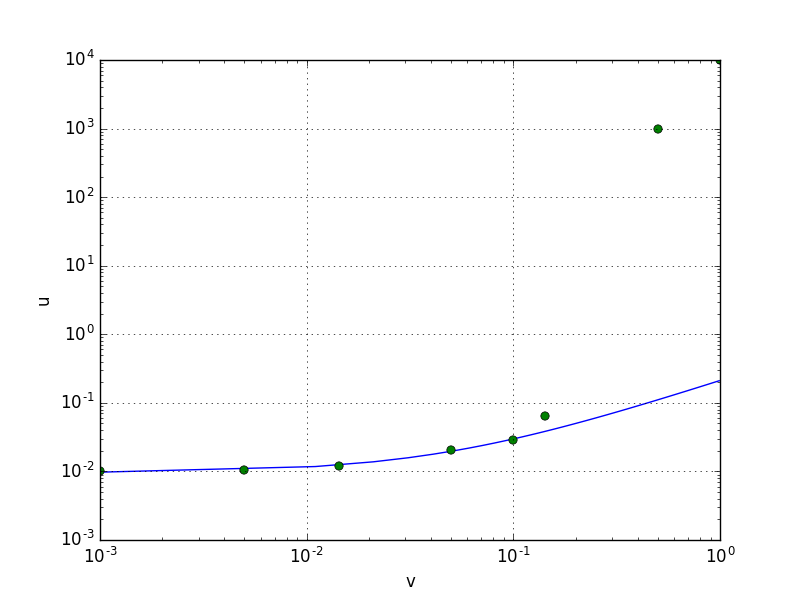
\includegraphics[scale=0.5]{slike/linarna2.png}
\hspace{\fill}
\end{flushleft}
\end{minipage}
\begin{minipage}[t]{0.5\paperwidth}
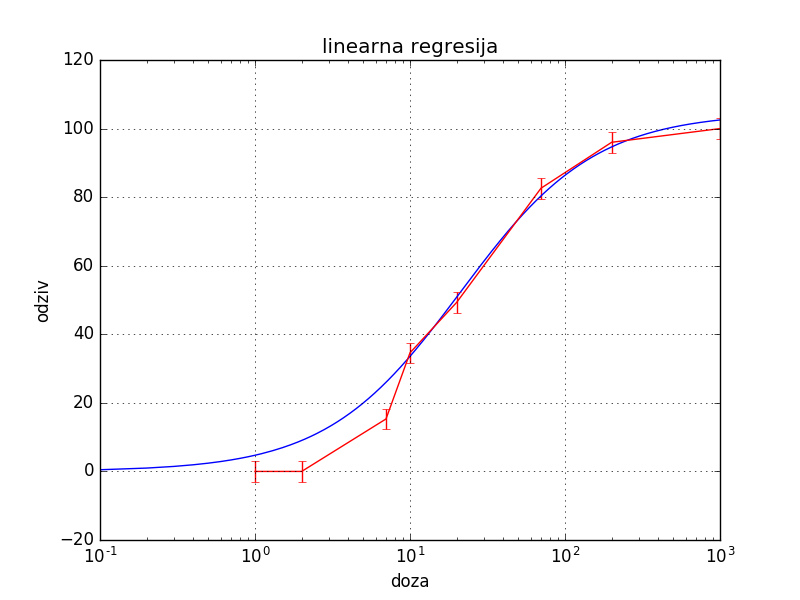
\includegraphics[scale=0.5]{slike/linearna1.png}
\end{minipage}%
}

\caption{Grafični prikaz rešitve. Na levi je linearna regresija na transformiranih podatkih, vendar sta obe osi v logaritemski skali. Na desni je prikaz meritev in njihova prilagoditvena funkcija.}
\end{figure}
\pagebreak

\section{Toplotna prevodnost jekla}

Imamo meritve toplotne prevodnosti jekla v odvisnosti od temperature in moči grelca:
  \begin{center}
    \begin{tabular}{r|c|lcr|c|l}
      $T$[$^\circ$F]&$P$[W]&$\lambda\rm[Btu/h\, ft\,^\circ F]$&\qquad\qquad&
      $T$[$^\circ$F]&$P$[W]&$\lambda\rm[Btu/h\, ft\,^\circ F]$\\
      \cline{1-3}\cline{5-7}
      100  &      545    &       41.60     &&      90   &     276    &   42.345\\
      161  &      602    &       37.7875   &&     149   &     275    &   39.5375\\
      227  &      538    &       36.4975   &&     206   &     274    &   37.3525\\
      270  &      550    &       35.785    &&     247   &     274    &   36.36\\
      362  &      522    &       34.53     &&     352   &     272    &   33.915
    \end{tabular}
  \end{center}
s podanimi napakami za meritve prevodnosti: $0.28$ za levo tabelo in $0.16$ za desno tabelo. Ker ne poznamo modela, ki bi nam opisal odvisnost prevodnosti od moči in temperature, opišemo prevodnost kot potenčno odvisnot oz. polinomsko.


\subsection{Osnovne potence}

Opis prevodnosti začnemo z preprostim polinomskim modelom:
\begin{equation*}
\lambda(T,P) = a_0 + \sum_{i=0}^n a_i T^i + \sum_{j=0}^m b_j P^j
\end{equation*}
pri čemer mora biti vsota $n+m$ manjša od $9$, saj z desetimi merilnimi točkami lahko določimo največ devet modelskih koeficientov. Ponovno lahko zgornjo enačbo zapišemo v matrično obliko, saj so relacije med koeficienti in prevodnostjo linearna. Ponovno iščemo minimum funkcije \ref{hi-minimum} in za reševanje koeficientov uporabimo enačbo \ref{resitev-koeficientov}. Ker ne vemo katera stopnja polinoma je optimalna poskusimo vse možnosti, pri čemer gresta $n$ in $m$ od nič do $n+m<9$. Sedaj moramo vrednosti $\chi^2$ primerno normalizirati, saj z vpeljavo dodatnih modelskih parametrov boljše opišemo naše meritve. Najlažje je uvesti dodatni parameter $\chi^2_{red}$, ki ga določimo:
\begin{equation*}
\chi^2_{red}=\frac{\chi^2}{N-M}
\end{equation*}
kjer je $N$ število merilnih točk in $M$ število modelskih parametrov.

\begin{figure}[ht]
\begin{center}
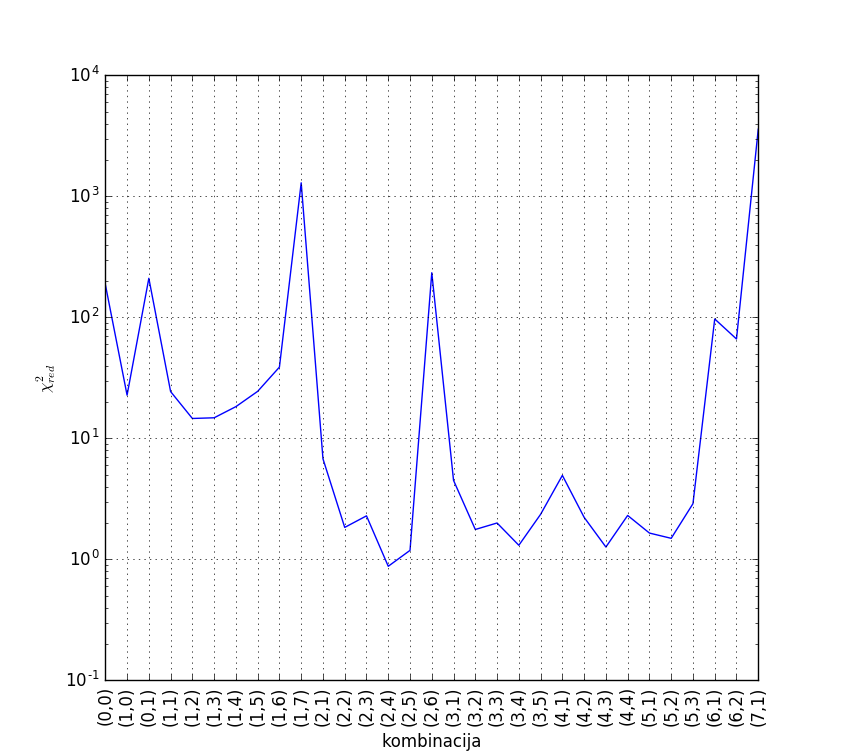
\includegraphics[scale=0.7]{slike/samo_potence_log.png}
\end{center}
\caption{Grafični prikaz vrednosti $\chi^2_{red}$, v primerjavi s kombinacijo $n$, $m$ (temperatura, moč). Opazimo zelo velike skoke vrednosti $\chi^2_{red}$ med posameznimi kombinacijami potenc. Vidimo, da model pri $m$ med $2$ in $4$ $\chi^2_{red}$ ne skače veliko, medtem ko za $n$ pa  $\chi^2_{red}$ se stabilizira od $2$ naprej. Iz grafa opazimo najboljši model z $n=2$ in $m=4$. }
\end{figure}


\subsection{Potence $TP$, $\frac{T}{P}$}
Predpostavimo, da zgornji model ne opiše dovolj dobro oz. imamo neposredno odvisnost moči in temperature. Sedaj uporabimo, dodatne člene $T^iP^j$, $\frac{T^i}{P^j}$ k opisu modela prevodnosti:

\begin{equation*}
\begin{aligned}
\lambda(T,P) &= a_0 + \sum_{i=0}^n a_i T^i + \sum_{j=0}^m b_j P^j +  c_k T P^k \\
\lambda(T,P) &= a_0 + \sum_{i=0}^n a_i T^i + \sum_{j=0}^m b_j P^j +  c_k P T^k
\end{aligned}
\end{equation*}
Za uporabo ulomka oz. členov $\frac{T}{P}$, smo pri zgornjih dveh enačbah potence dodatnega člena negirali. Na naslednji strani je prikaz zgornjih dveh enačb, naslednja stran pa ko smo potence dodatnega člena negirali.



\begin{sidewaysfigure}
\begin{center}
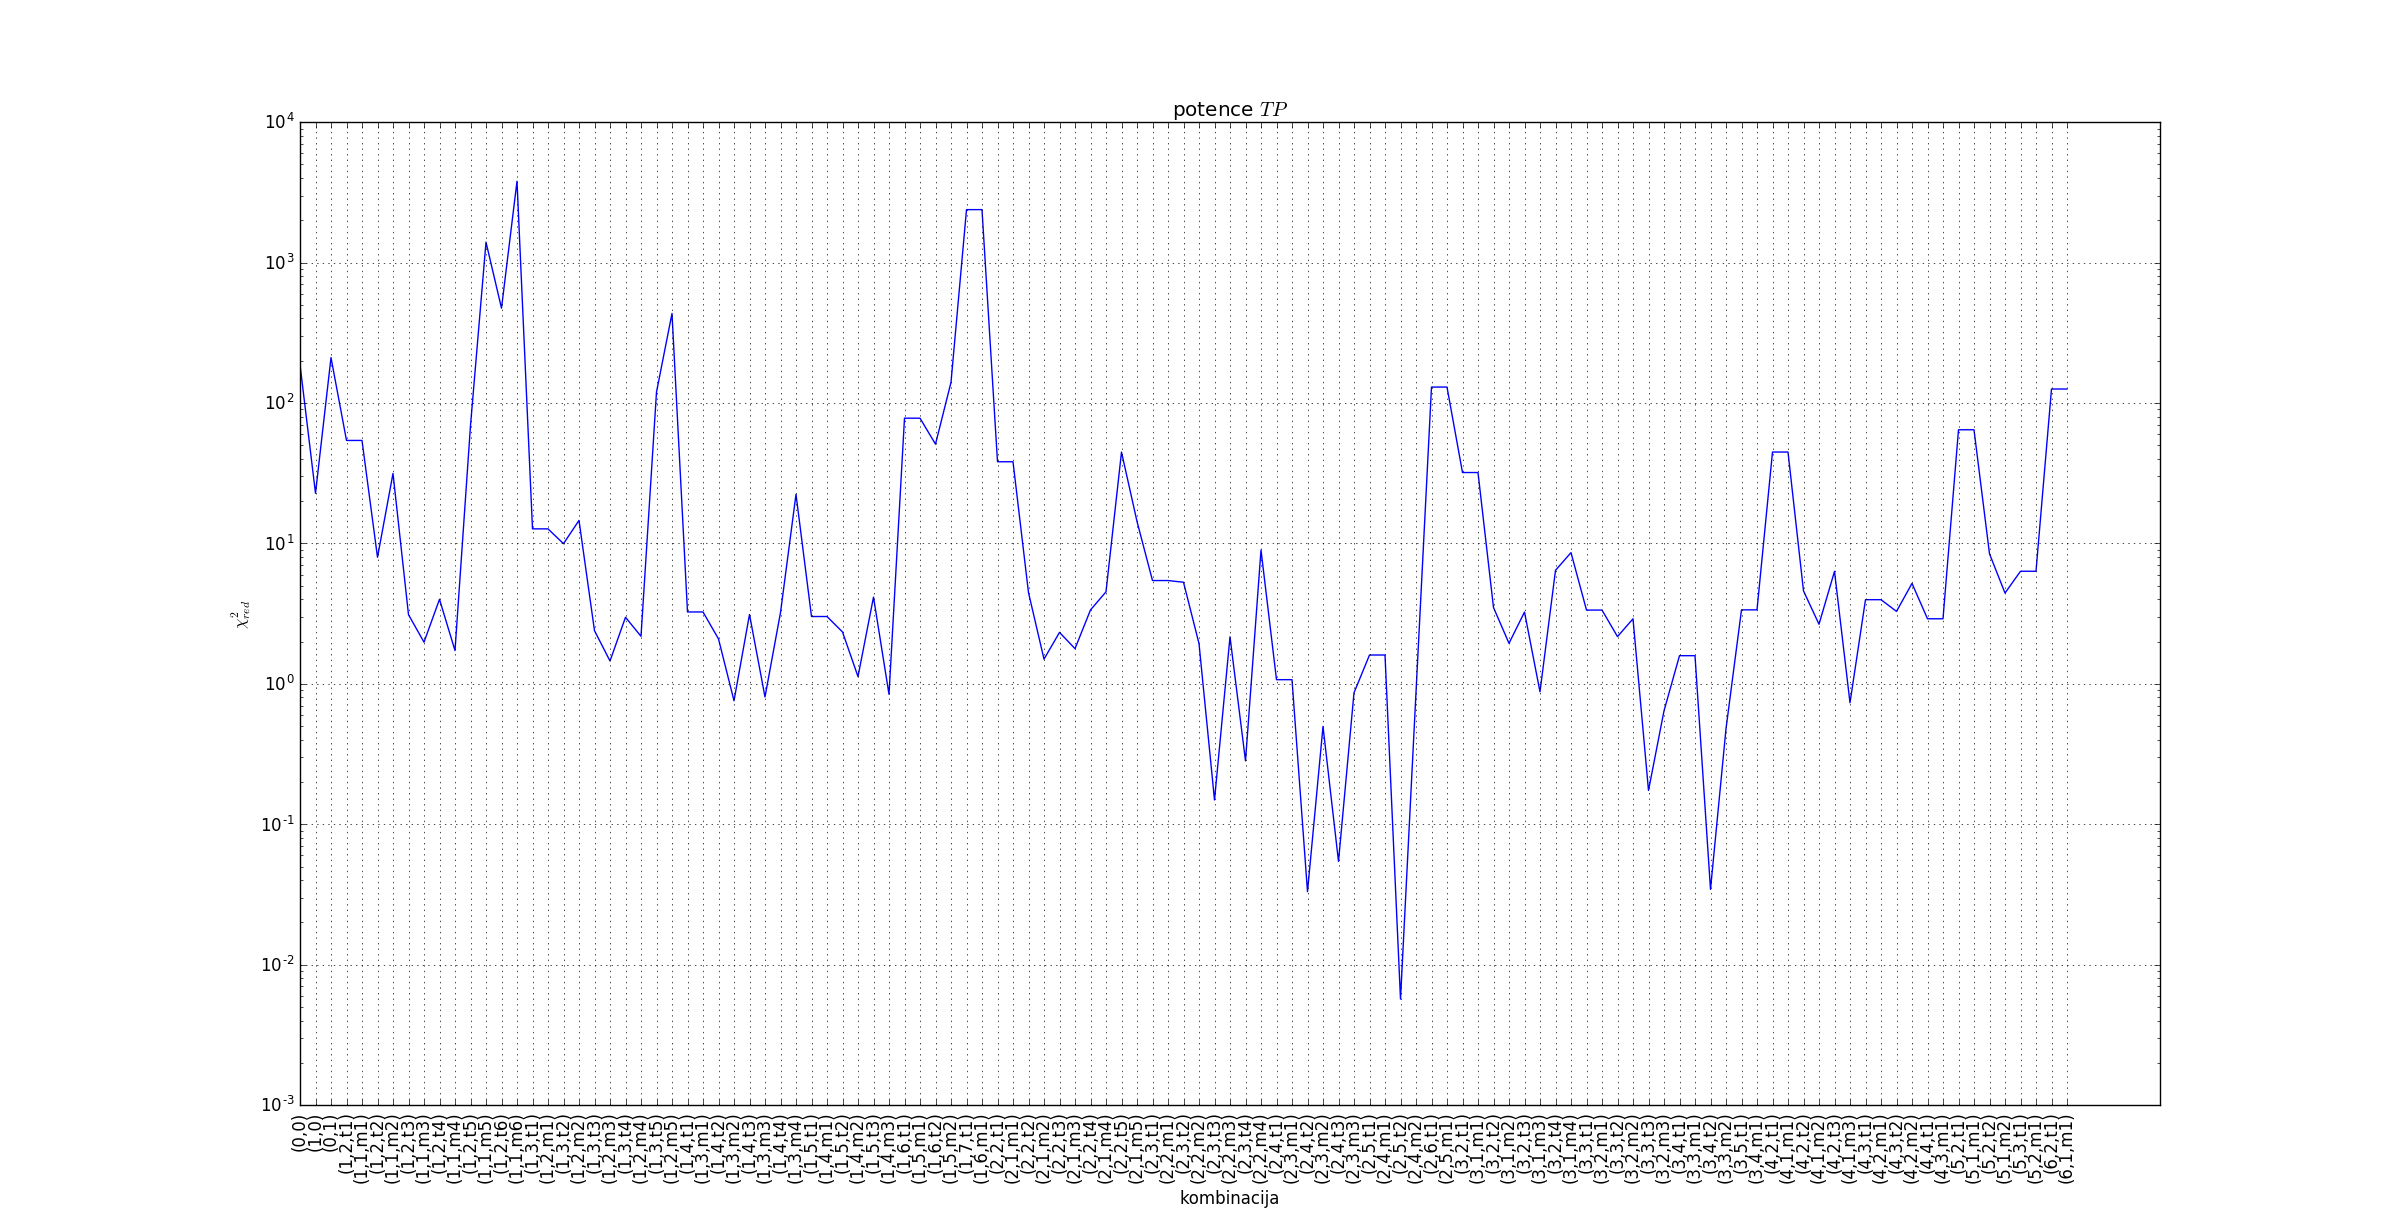
\includegraphics[scale=0.5]{slike/samo_potence_log_tp.png}
\caption{V prejšnjem poglavju, kjer smo imeli le osnovne potence moči in temperature, je $\chi_{red}^2$ imel vrednost $0.877$ pri najbolšem modelu. Tokrat opazimo, da imajo vrednosti $\chi_{red}^2$ veliko večji razpon. Imamo pa $16$ kombinacij, ki boljše opišejo kot model z osnovnimi potencami. Občutno najboljše opiše model ($\chi_{red}^2$ je v tem primeru $0.00569$ in je za dva velikostna razreda manjša), ki ima osnovno potence temperature $2$, moči $5$ ter dodatni člen $PT^2$.}
\end{center}
\end{sidewaysfigure}

\begin{sidewaysfigure}
\begin{center}
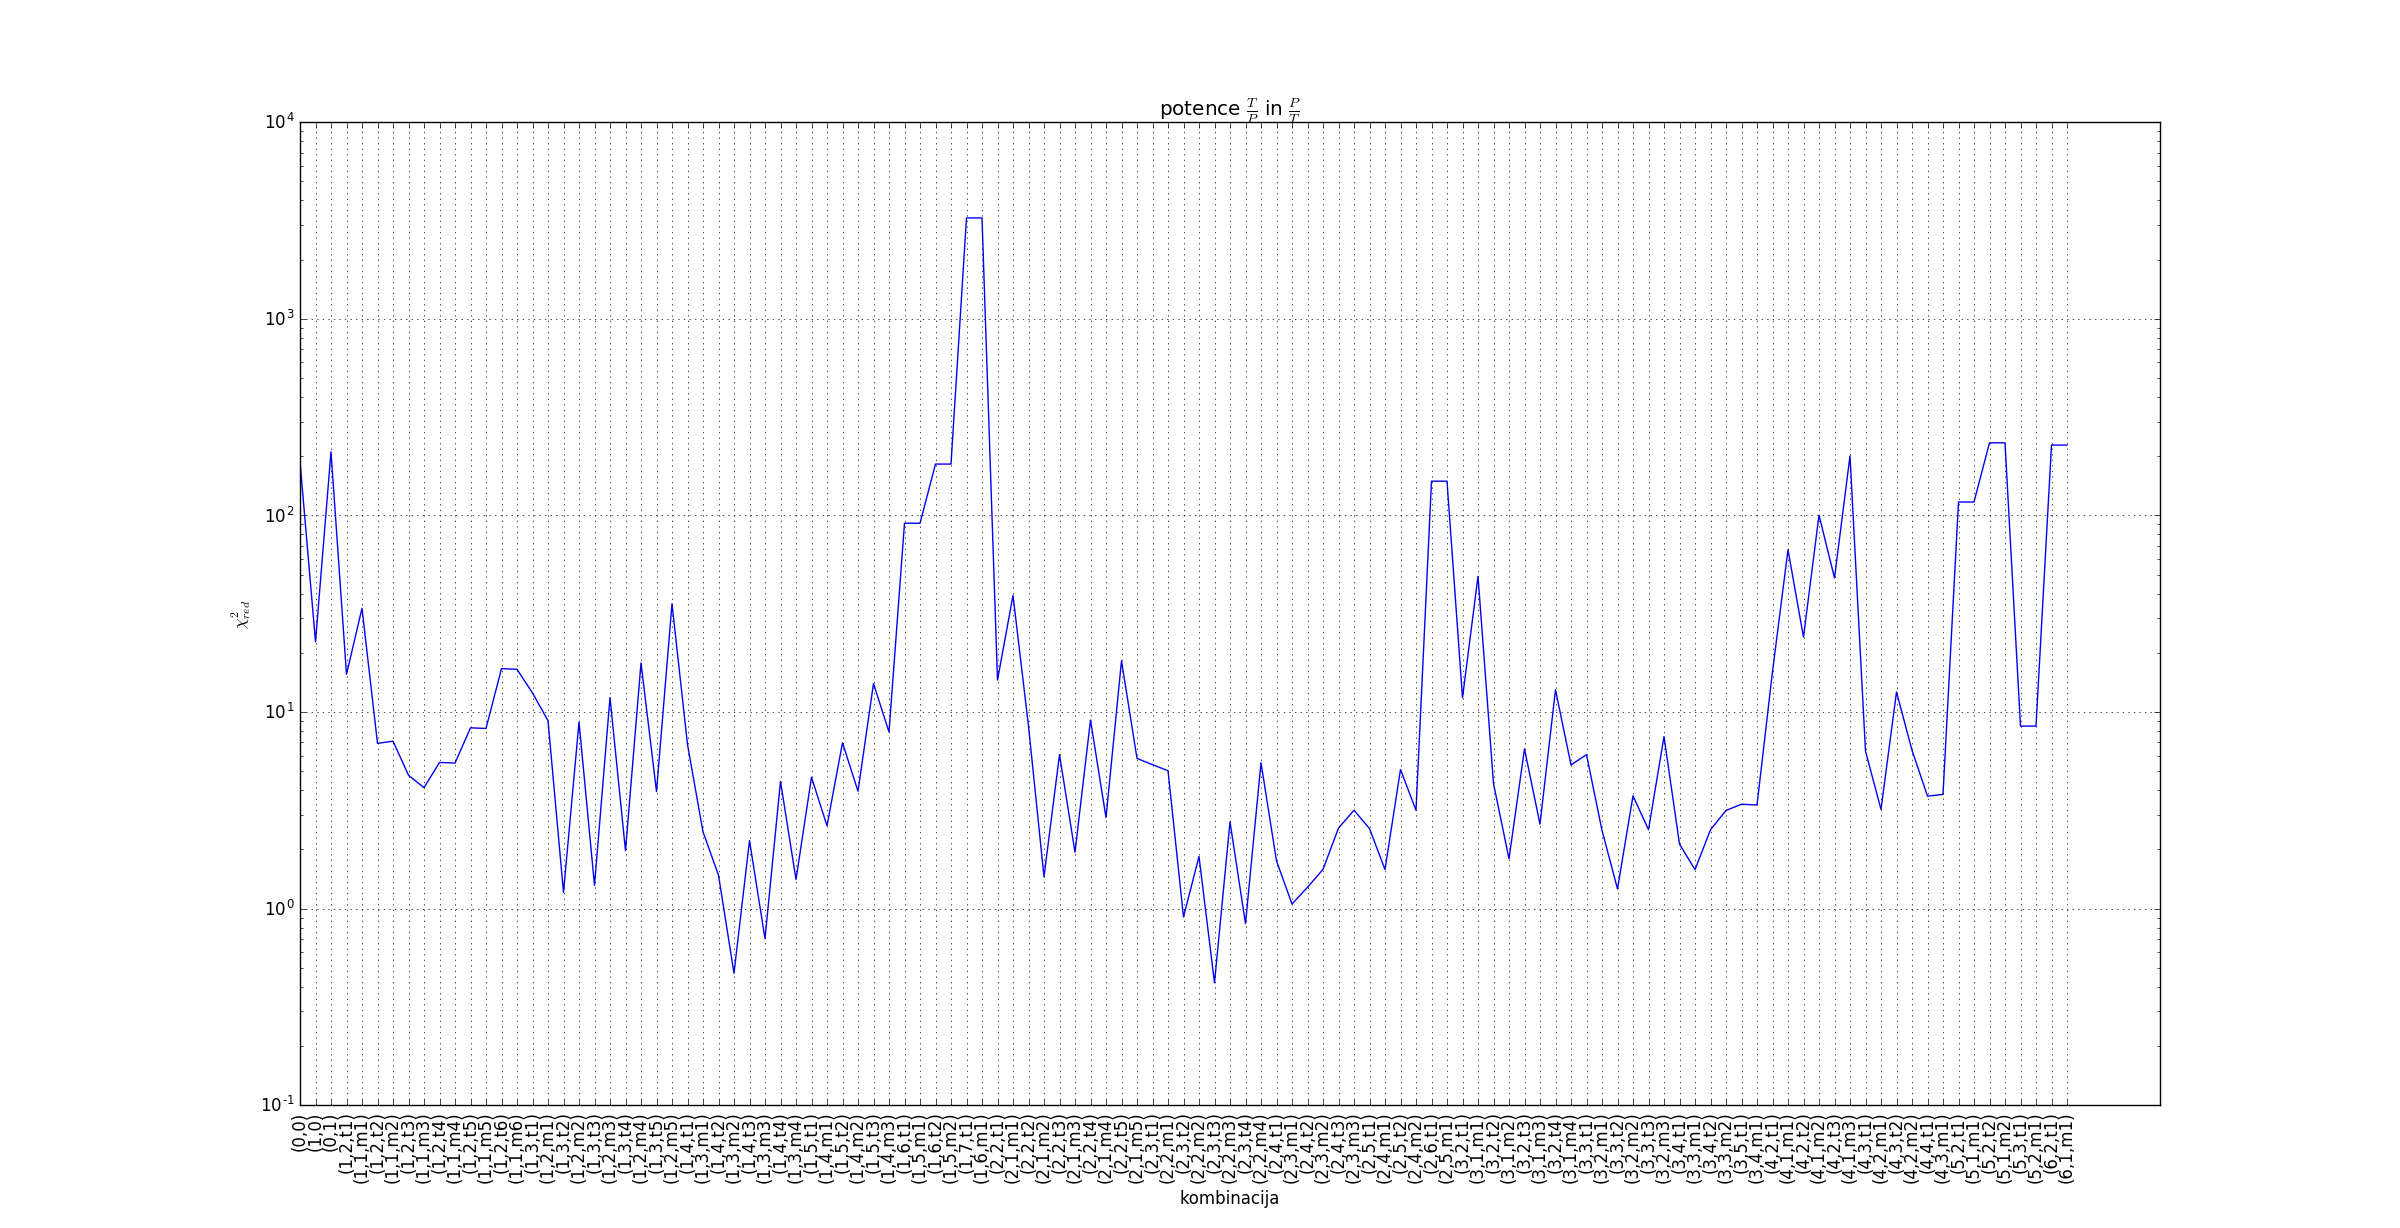
\includegraphics[scale=0.5]{slike/samo_potence_log_ulomki.png}
\caption{Z vpeljavo členov $\frac{T}{P^i}$ in $\frac{P}{T^i}$ dobimo od najboljšega osnovnega modela le $4$ boljše modele, ki pa niso občutno boljši od osnovnega modela. }
\end{center}
\end{sidewaysfigure}

\section{Profil rentgenskih robov}

Imamo profila absorpcije rentgenskih žarkov izoliranih sten iz krovne plasti in sredice listov rastline \textit{C. Thlaspi}. Zanima nas razmerje med vezi Cd-O in Cd-S v obeh profilih. Za obliko profila absorpcije rentgenskih žarkov uporabimo standarde, ki smo jih dobili iz GSH za Cd-S in iz pektinoma za Cd-O. 	


\begin{figure}[ht]
\noindent\makebox[\textwidth][l]{%
\hspace{-\dimexpr\oddsidemargin+1in}%

\begin{minipage}[t]{0.5\paperwidth}
\begin{flushleft}
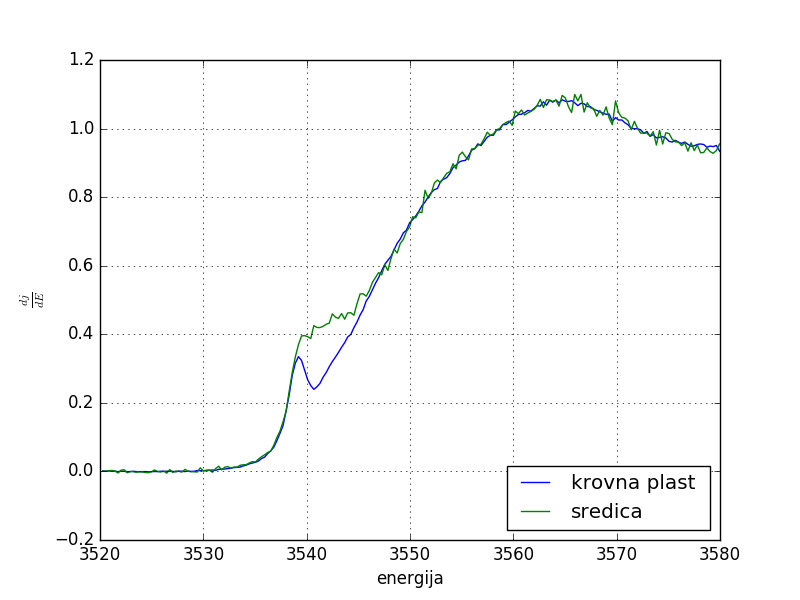
\includegraphics[scale=0.5]{slike/meritve_specter.png}
\hspace{\fill}
\end{flushleft}
\end{minipage}
\begin{minipage}[t]{0.5\paperwidth}
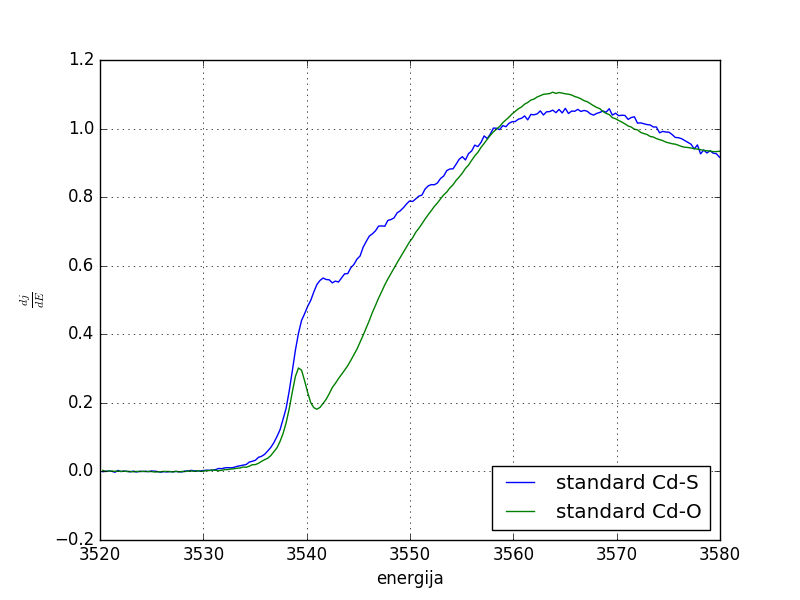
\includegraphics[scale=0.5]{slike/standard_specter.png}
\end{minipage}%
}

\caption{Na levem grafu imamo meritve absorpcije rentgenskih žarkov na dveh različnih vzorcih lista. Iz standardov, ki ga ponazarja desni graf moramo določiti odstotno razmerje vezi Cd-O in Cd-S v vzorcema. }
\end{figure}

najprej moramo določiti koliko je posameznih vezi v vzorcu. To najlažje določimo tako da je rezultat meritev linearna kombinacija standardov:
\begin{equation}
\begin{aligned}
\frac{dj}{dE} \Big|_1 &= a_1 S_1 + a_2 S_2 \\
\frac{dj}{dE} \Big|_2 &= b_1 S_1 + b_2 S_2
\end{aligned}
\end{equation}
kjer je $\frac{dj}{dE}$ meritve absorpcije rentgenskih žarkov, $S$ meritev absorpcije na standardu ter koeficienti $a$, $b$ do neznanega faktorja število vezi danega standarda. Ponovno zgornji enačbi lahko preoblikujemo v matrično obliko in rešujemo kot v zgornjih nalogah. Za odstotno razmerje v posameznem vzorcu delimo prvi koeficient z drugim. 

  \begin{center}
    \begin{tabular}{r|c|lcr|c|l}
      &vrednost &napaka\\
      \cline{1-3}
      $a_1$  &      0.2727    &       0.009\\
      $a_2$  &      0.7301    &       0.009\\
      $r_1= \frac{a_1}{a_2}$  &      0.3735    &       0.013\\
      $b_1$ &      0.5544    &       0.012\\
      $b_2$  &      0.4459    &       0.013\\
       $r_2= \frac{b_1}{b_2}$  &      1.243    &       0.036
    \end{tabular}
  \end{center}

Oglejmo si že absolutno razliko med linearnim prilagajanjem in meritvami.

\begin{figure}[ht]
\begin{center}
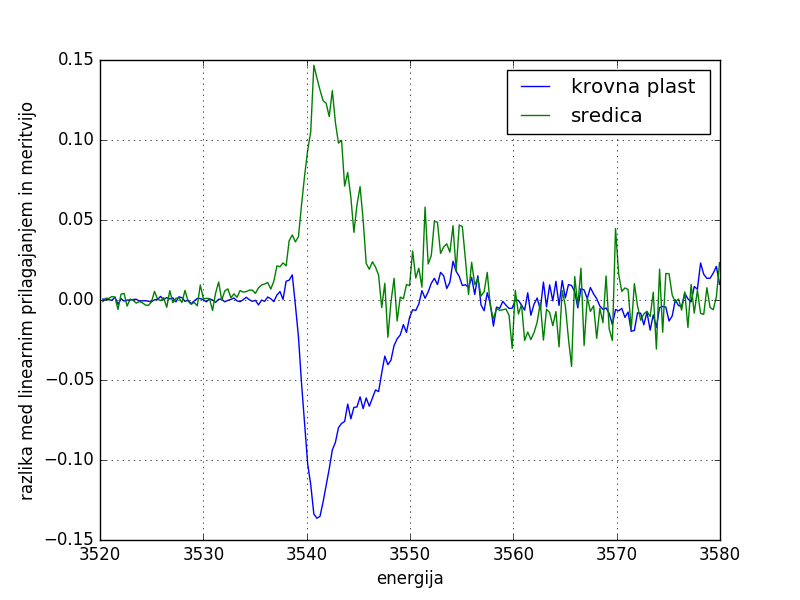
\includegraphics[scale=0.7]{slike/razlika_spekter.png}
\end{center}
\caption{Če pogledamo vrednosti koeficientov vidimo, da so napake velike nekaj procentov (do max $5\%$), kar nam lahko pove, da bo je to dobro prilagajanje. Sedaj pa si oglejmo razliko med prilagojeno krivuljo in meritvami. Opazimo za oba vzorca opazno odstopanje pri enaki energiji. Če pogledamo standarde, opazimo da je največje odstopanje ravno v lokalnem minimumu standardov. Torej bo potrebno naš model še bolje izpopolniti. Ena možnost je, da pri meritvi sredice lista poskušamo zgladiti meritev, vendar to še vedno ne bo odstranilo izrazitega vrha. Naslednja možnost in najverjetnejša, je da je potrebno k standardom upoštevati še nek dodaten člen.}
\end{figure}


%-------------------------------------------------------------------------------------------




\end{document}
